\usetikzlibrary{trees}
% \tikzstyle{level 1}=[level distance=2cm, sibling distance=4cm]
% \tikzstyle{level 2}=[level distance=2cm, sibling distance=1cm]
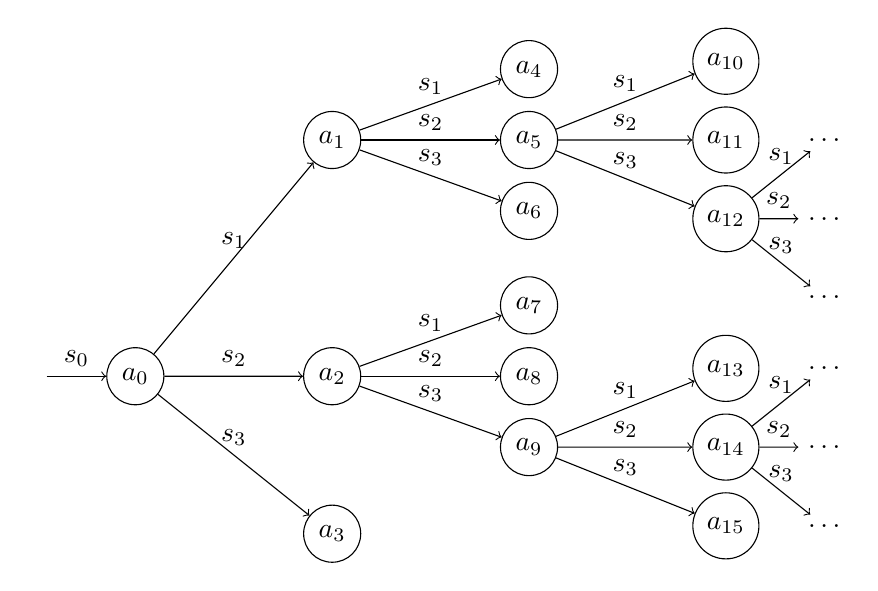
\begin{tikzpicture}[
        grow=right,
        ->,
        % every node/.style={draw,circle},
        state/.style={draw, circle},
        % treenode/.style = {circle, white, draw=black, align=center, inner sep=0pt, text centered, font=\sffamily},
        % thick,
        % Set the overall layout of the tree
        level/.style={level distance=2.5cm},
        level 1/.style={level distance=1.25cm},
        level 2/.style={sibling distance=3cm},
        level 3/.style={sibling distance=0.9cm},
        level 4/.style={sibling distance=1cm},
        level 5/.style={level distance=1.25cm},
        % level/.style={sibling distance = 5cm/#1, level distance = 1.5cm}
    ]
    \node {}
    child {
        node [state] {$a_0$}
        child [sibling distance=2cm] {
            node [state] {$a_3$}
            edge from parent node [above] {$s_3$}
        }
        child {
            node [state] {$a_2$}
            child {
                node [state] {$a_9$}
                child {
                    node [state] {$a_{15}$}
                    edge from parent node [above] {$s_3$}
                }
                child {
                    node [state] {$a_{14}$}
                    child {
                        node {$\ldots$}
                        edge from parent node [above] {$s_3$}
                    }
                    child {
                        node {$\ldots$}
                        edge from parent node [above] {$s_2$}
                    }
                    child {
                        node {$\ldots$}
                        edge from parent node [above] {$s_1$}
                    }
                    edge from parent node [above] {$s_2$}
                }
                child {
                    node [state] {$a_{13}$}
                    edge from parent node [above] {$s_1$}
                }
                edge from parent node [above] {$s_3$}
            }
            child {
                node [state] {$a_8$}
                edge from parent node [above] {$s_2$}
            }
            child {
                node [state] {$a_7$}
                edge from parent node [above] {$s_1$}
            }
            edge from parent node [above] {$s_2$}
        }
        child {
            node [state] {$a_1$}
            child {
                node [state] {$a_6$}
                edge from parent node [above] {$s_3$}
            }
            child {
                node [state] {$a_5$}
                child {
                    node [state] {$a_{12}$}
                                        child {
                        node {$\ldots$}
                        edge from parent node [above] {$s_3$}
                    }
                    child {
                        node {$\ldots$}
                        edge from parent node [above] {$s_2$}
                    }
                    child {
                        node {$\ldots$}
                        edge from parent node [above] {$s_1$}
                    }
                    edge from parent node [above] {$s_3$}
                }
                child {
                    node [state] {$a_{11}$}
                    edge from parent node [above] {$s_2$}
                }
                child {
                    node [state] {$a_{10}$}
                    edge from parent node [above] {$s_1$}
                }
                edge from parent node [above] {$s_2$}
            }
            child {
                node [state] {$a_4$}
                edge from parent node [above] {$s_1$}
            }
            edge from parent node [above] {$s_1$}
        }
        edge from parent node [above] {$s_0$}
    };
\end{tikzpicture}

% \begin{tikzpicture}[
%         ->,
%         every node/.style={draw,circle},
%         % treenode/.style = {circle, white, draw=black, align=center, inner sep=0pt, text centered, font=\sffamily},
%         thick,
%         % Set the overall layout of the tree
%         level/.style={level distance=1.5cm},
%         level 2/.style={sibling distance=2.6cm},
%         level 3/.style={sibling distance=2cm}
%     ]
%     \coordinate
%         child[grow=left]{
%             node {$a_0$}
%             % node [treenode] {$a_0$}
%             edge from parent node [above=3pt] {$s_0$}
%         }
%         % I have to insert a dummy child to get the tree to grow
%         % correctly to the right.
%         child[grow=right, level distance=0pt] {
%         node [above] {$a_1$}
%         child  {
%             child {
%                 child {
%                     node {$\bar{d}$}
%                     edge from parent
%                 }
%                 child {
%                     node {$u$}
%                     edge from parent
%                 }
%                 edge from parent
%             }
%             child {
%                 node {$b$}
%                 edge from parent
%             }
%             edge from parent
%             node [below] {$t$}
%         }
%         child {
%             child {
%                 node {$\bar{b}$}
%                 edge from parent
%             }
%             child {
%                 child {
%                     node {$\bar{v}$}
%                     edge from parent
%                 }
%                 child {
%                     node {$e^{-}$}
%                     edge from parent
%                 }
%                 edge from parent
%             }
%             edge from parent
%             node [above] {$\bar{t}$}
%         }
%     };
% \end{tikzpicture}